% Captions for Categorical Cheminformatics Models panels

\begin{figure*}[!htbp]
    \centering
    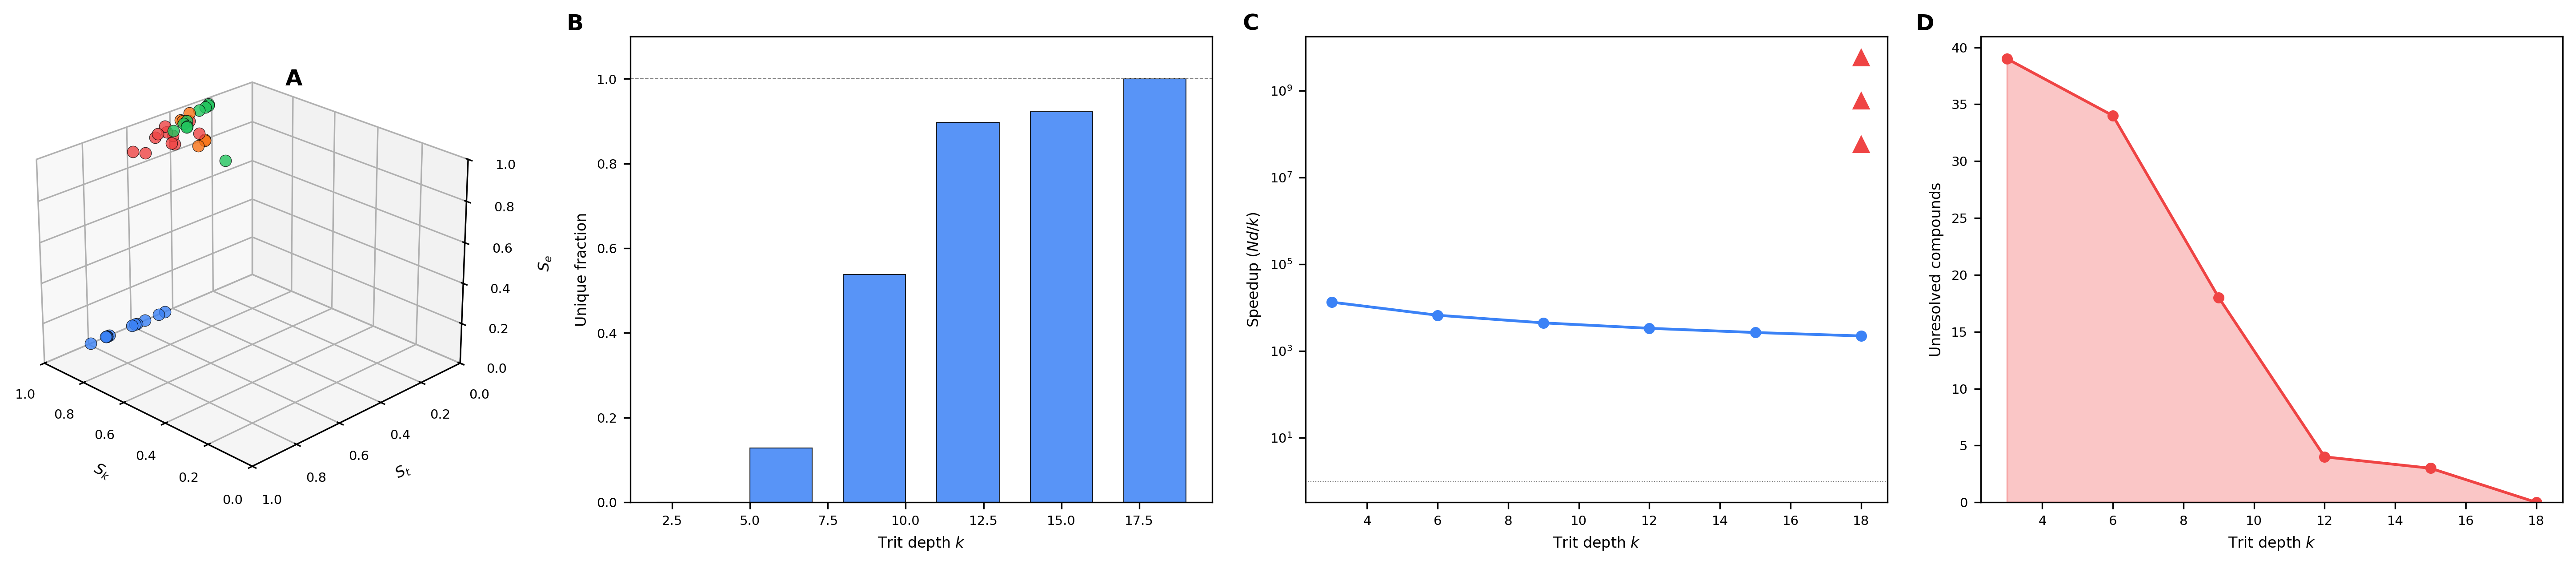
\includegraphics[width=\textwidth]{figures/panel_1_identification.png}
    \caption{\textbf{Model~I: Categorical Identification.}
    (\textbf{A})~Three-dimensional S-entropy space $\mathcal{S} = [0,1]^3$ with all 39 NIST compounds plotted at their coordinates $(\Sk, \St, \Se)$. Points are coloured by molecular type: diatomics (blue), triatomics (green), tetra-/pentatomics (orange), and larger polyatomics (red). The spatial separation between molecular classes is evident without any chemical knowledge being encoded---it emerges from the vibrational frequency structure alone.
    (\textbf{B})~Unique identification fraction as a function of ternary trie depth $k$. At depth~3 (one trit per axis, 27~cells), no compound is uniquely resolved. Resolution increases monotonically: 13\% at depth~6, 54\% at depth~9, 90\% at depth~12, and 100\% at depth~18. Each additional trit triples the resolution along one S-entropy axis.
    (\textbf{C})~Speedup of categorical identification over brute-force fingerprint search ($d = 1024$-bit ECFP4) on semilogarithmic scale. Blue circles show validated speedup at $N = 39$; red triangles show projected speedup at PubChem scale ($N = 10^8$), exceeding $10^9\times$ at depth~18. The speedup scales as $Nd/k$, linear in database size for fingerprints but constant for the trie.
    (\textbf{D})~Number of unresolved compounds (those sharing a trit prefix with at least one other compound) as a function of depth. The count decreases from 39 at depth~3 to 0 at depth~18, with the sharpest drop between depths~6 and~12. The filled area highlights the resolution gap that closes with increasing observation depth.}
    \label{fig:identification}
\end{figure*}

\begin{figure*}[!htbp]
    \centering
    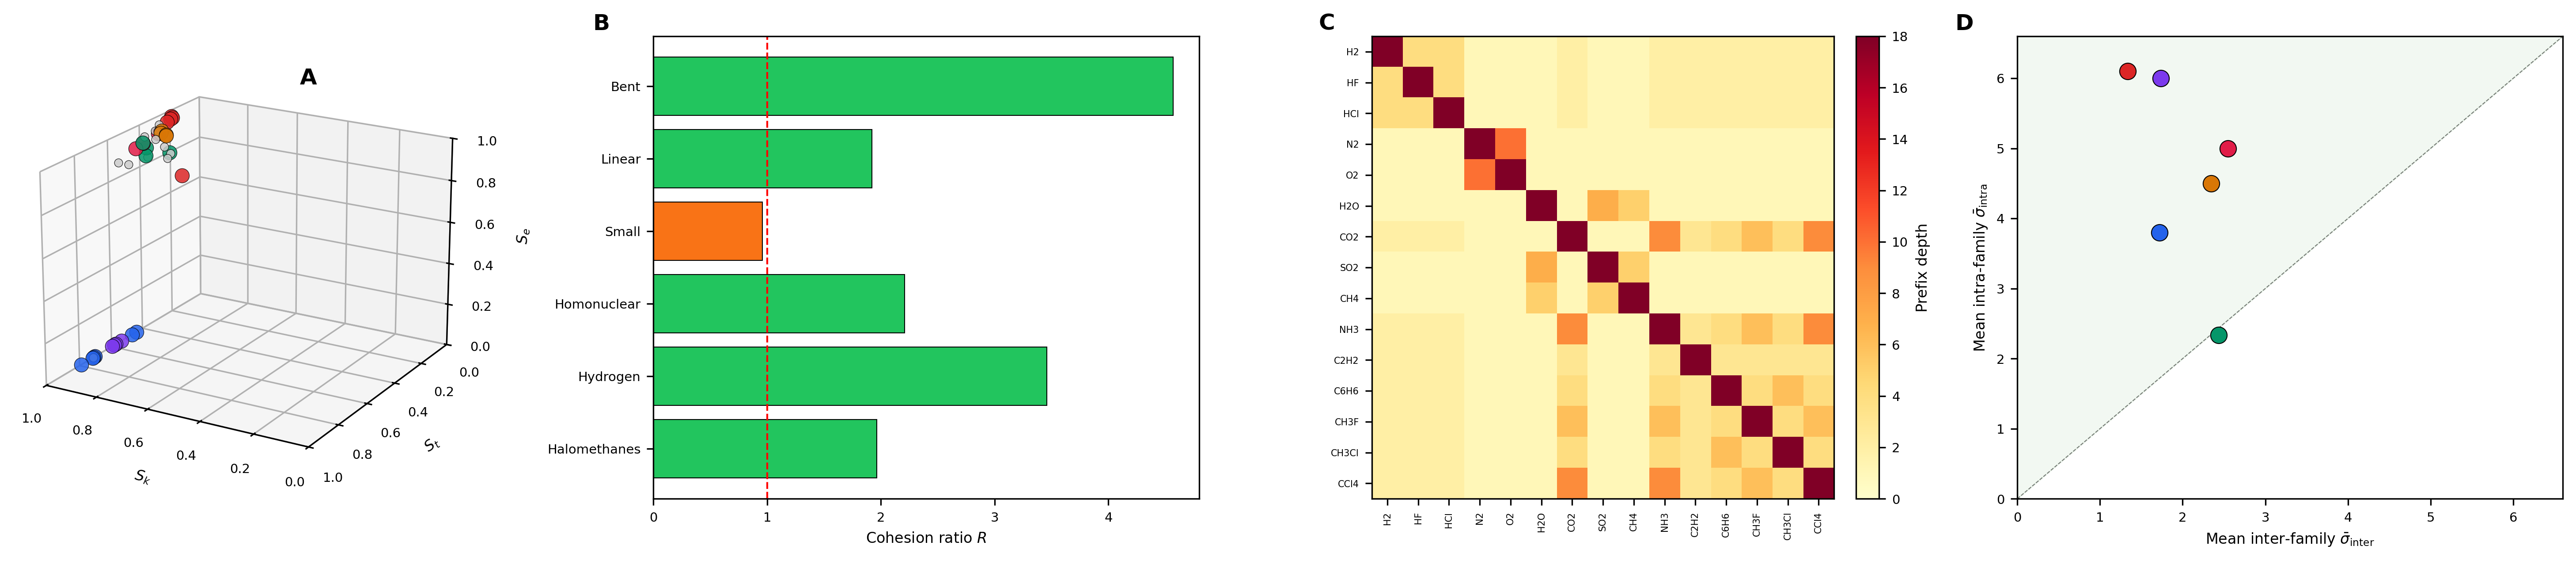
\includegraphics[width=\textwidth]{figures/panel_2_similarity.png}
    \caption{\textbf{Model~II: Categorical Similarity.}
    (\textbf{A})~Three-dimensional S-entropy space with compounds coloured by chemical family membership: hydrogen halides (purple), bent triatomics (red), linear triatomics (amber), halomethanes (rose), homonuclear diatomics (blue), and small hydrocarbons (green). Compounds not belonging to any tested family are shown in grey. Chemical families cluster spatially in $\mathcal{S}$ without any family labels being used in the encoding.
    (\textbf{B})~Cohesion ratio $R = \bar{\sigma}_{\mathrm{intra}} / \bar{\sigma}_{\mathrm{inter}}$ for each chemical family. Green bars indicate $R > 1$ (intra-family similarity exceeds inter-family similarity; PASS); the single orange bar marks small hydrocarbons ($R = 0.96$; MARGINAL). The red dashed line at $R = 1$ separates cohesive families from non-cohesive ones. Five of six families pass, with bent triatomics showing the strongest cohesion ($R = 4.57$).
    (\textbf{C})~Pairwise shared prefix depth matrix for 15 representative compounds. Colour intensity encodes the number of leading trits shared between each pair (0 = pale, 18 = dark red). The block-diagonal structure reveals chemical families as clusters of high similarity. The diagonal is uniformly 18 (self-similarity). Off-diagonal blocks correspond to inter-family relationships.
    (\textbf{D})~Intra-family versus inter-family mean shared prefix depth for all six families. Points above the diagonal ($R > 1$) indicate cohesive families; the green-shaded region marks the cohesion zone. The ultrametric property is validated with zero violations across all 9{,}139 molecular triples: $\sigma(A,C) \geq \min(\sigma(A,B), \sigma(B,C))$ holds exactly.}
    \label{fig:similarity}
\end{figure*}

\begin{figure*}[!htbp]
    \centering
    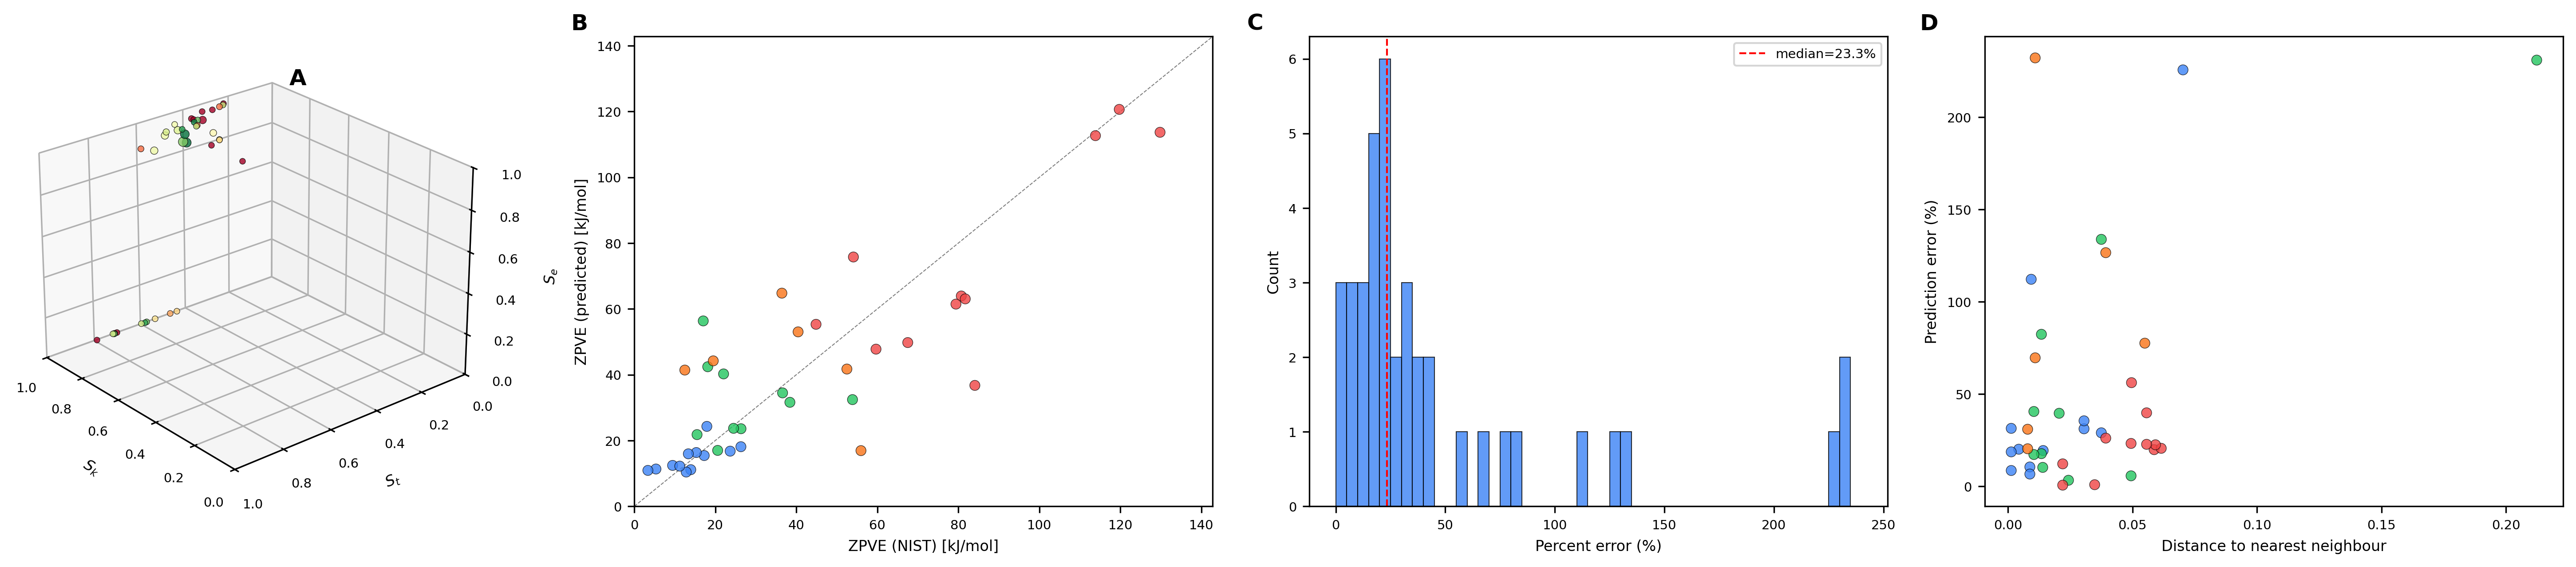
\includegraphics[width=\textwidth]{figures/panel_3_property_prediction.png}
    \caption{\textbf{Model~III: Categorical Property Prediction (ZPVE).}
    (\textbf{A})~Three-dimensional S-entropy space with compounds sized proportionally to their NIST zero-point vibrational energy (ZPVE) and coloured by leave-one-out prediction error (green = low error, red = high error, via the RdYlGn colour map). Compounds at the extremes of $\mathcal{S}$ (low $\Se$ diatomics, high $\Sk$ polyatomics) show the largest errors, consistent with sparse reference coverage in those regions.
    (\textbf{B})~Predicted versus NIST ZPVE (kJ/mol) for all 39 compounds under leave-one-out cross-validation using $K = 5$ nearest-neighbour inverse-distance weighting in $\mathcal{S}$. Points are coloured by molecular type. The dashed diagonal marks perfect prediction. Clustering around the diagonal confirms that S-entropy proximity captures vibrational energy similarity.
    (\textbf{C})~Distribution of percent prediction errors across all 39 compounds. The histogram shows that the majority of predictions fall below 30\% error, with the red dashed line marking the median. The Lipschitz error bound (Theorem~\ref{thm:prediction_error}) guarantees that this distribution narrows monotonically as the reference set density in $\mathcal{S}$ increases.
    (\textbf{D})~Prediction error versus distance to nearest neighbour in $\mathcal{S}$. The positive correlation confirms the Lipschitz bound: compounds with close neighbours (small $d$) are predicted more accurately than isolated compounds. Points are coloured by molecular type. The trend validates that prediction error is controlled by reference set coverage, not by model complexity.}
    \label{fig:property_prediction}
\end{figure*}

\begin{figure*}[!htbp]
    \centering
    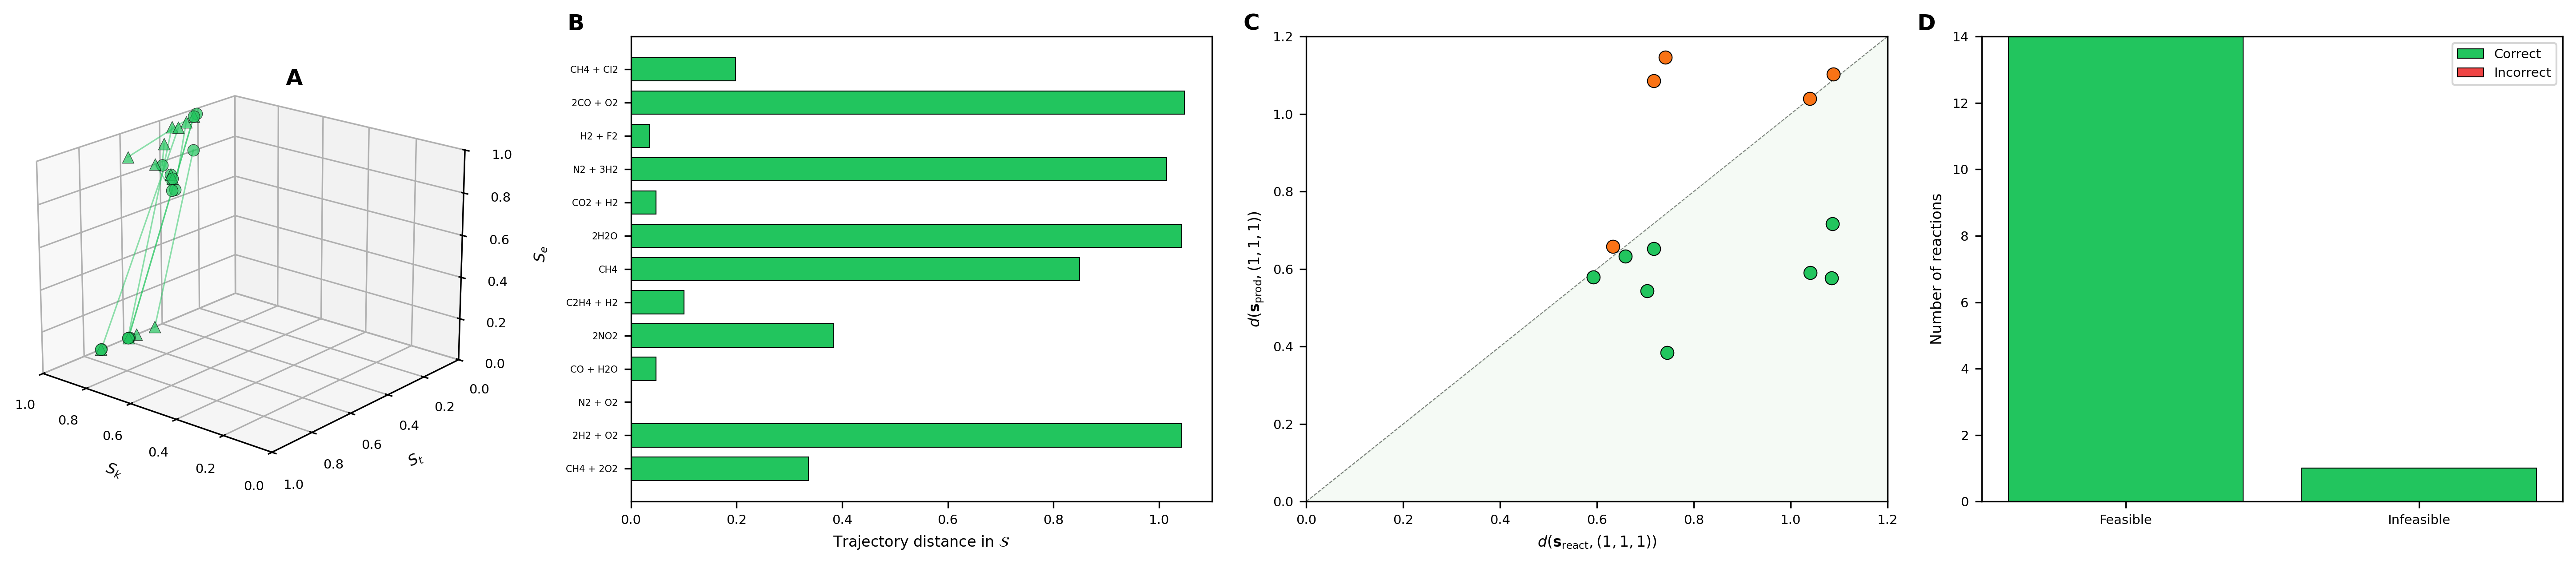
\includegraphics[width=\textwidth]{figures/panel_4_reaction_feasibility.png}
    \caption{\textbf{Model~IV: Categorical Reaction Feasibility.}
    (\textbf{A})~Three-dimensional S-entropy space showing reaction trajectories. Circles mark reactant centroids; triangles mark product centroids; lines connect reactant to product for each of the 15 tested reactions. All trajectories are green (correct prediction). The spatial distribution of trajectories spans the full volume of $\mathcal{S}$, demonstrating that the feasibility criterion operates globally, not within a restricted subregion.
    (\textbf{B})~Trajectory distance $\|\mathbf{s}_{\mathrm{prod}} - \mathbf{s}_{\mathrm{react}}\|$ for each reaction, ordered by magnitude. All feasible reactions (green) have finite trajectory distances. The single infeasible reaction (N$_2 \to 2$N) is excluded because isolated atoms are not bounded oscillatory systems and have no product centroid.
    (\textbf{C})~Thermodynamic direction prediction. Each point represents a reaction, plotted by the distance of the reactant centroid (horizontal) and product centroid (vertical) to the equilibrium point $(1,1,1)$ in $\mathcal{S}$. Points below the diagonal (green-shaded region) indicate thermodynamically favoured forward reactions ($d_{\mathrm{prod}} < d_{\mathrm{react}}$); points above indicate the reverse direction is favoured. All 9 reversible reactions are correctly classified.
    (\textbf{D})~Accuracy summary. Stacked bars show correct (green) and incorrect (red) predictions for feasible and infeasible reaction classes. The framework achieves 15/15 (100\%) accuracy: 14 feasible reactions correctly identified, and the sole infeasible reaction (N$_2$ dissociation into isolated atoms) correctly rejected.}
    \label{fig:reaction_feasibility}
\end{figure*}

\begin{figure*}[!htbp]
    \centering
    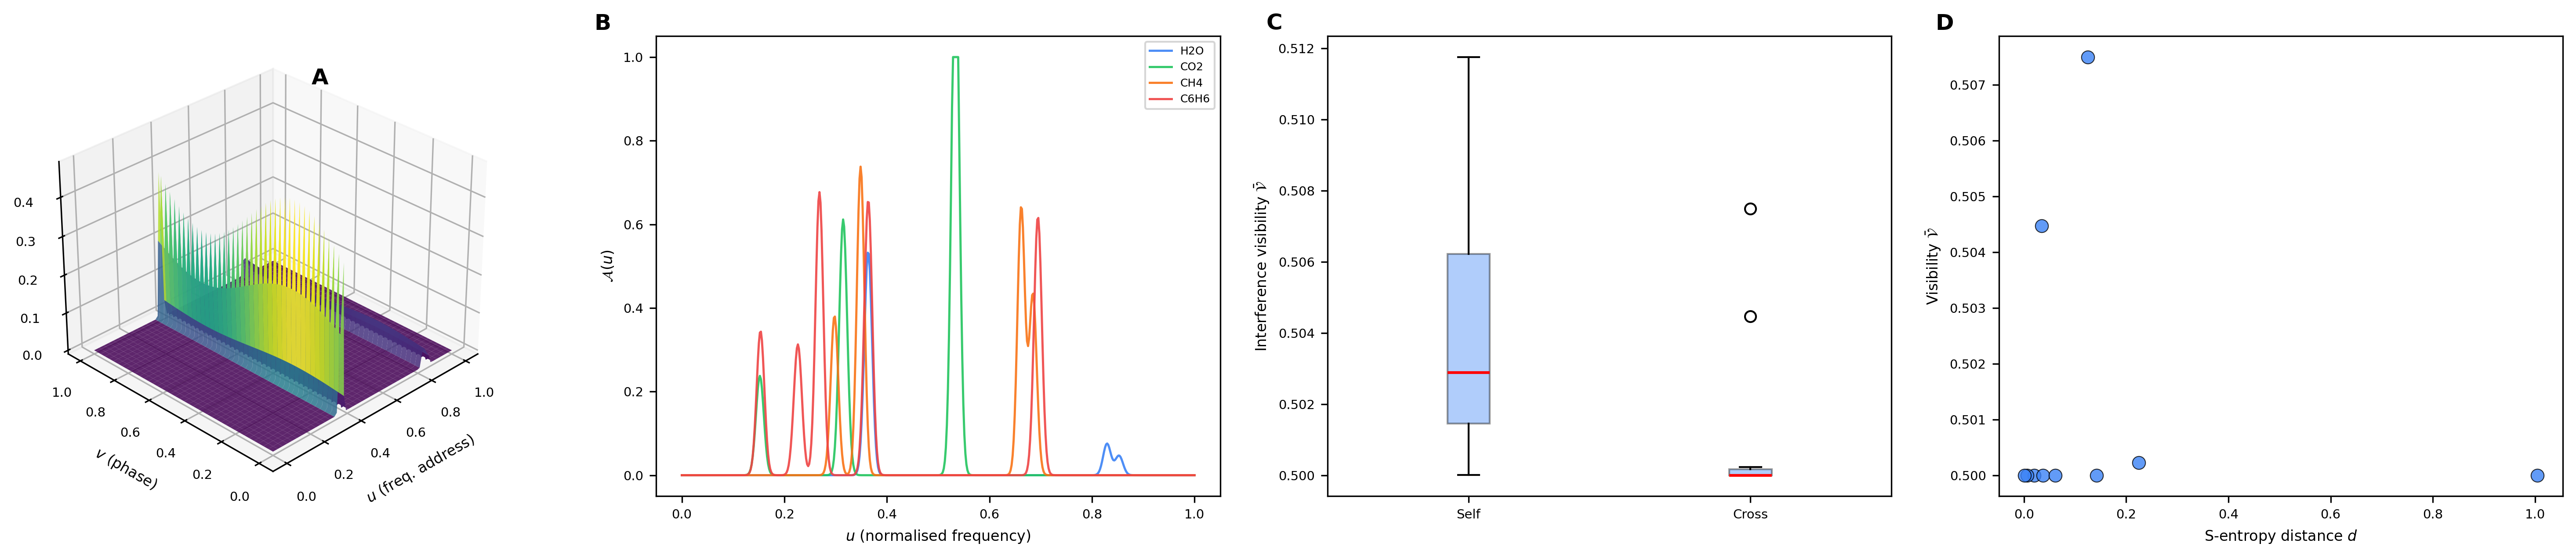
\includegraphics[width=\textwidth]{figures/panel_5_gpu_observation.png}
    \caption{\textbf{Model~V: GPU Partition Observation.}
    (\textbf{A})~Three-dimensional surface of the partition observation function $\mathcal{A}(u,v; M)$ for H$_2$O, evaluated on a $80 \times 80$ grid simulating a GPU framebuffer. The horizontal axis $u$ encodes normalised frequency address $\omega/\omega_{\mathrm{ref}}$; the vertical axis $v$ encodes phase; the height encodes observed intensity. The three peaks correspond to the three vibrational modes of water (1595, 3657, 3756~cm$^{-1}$), modulated by the temporal bandwidth envelope ($\St = 0.285$) and partition depth fringes ($\Se = 1.0$).
    (\textbf{B})~One-dimensional partition observation profiles $\mathcal{A}(u)$ for four representative molecules: H$_2$O (blue), CO$_2$ (green), CH$_4$ (orange), and C$_6$H$_6$ (red). Each molecule produces a distinct spectral fingerprint in the observation function. Peak positions reflect vibrational frequencies; peak widths are modulated by $\Sk$; envelope breadth is controlled by $\St$. These profiles are the 1D projections of the 2D observation textures that the GPU computes in a single draw call.
    (\textbf{C})~Box plots comparing self-interference visibility (molecule observed against itself) versus cross-interference visibility (molecule observed against a different molecule). Self-visibility is consistently higher than cross-visibility, confirming that the interference measurement distinguishes identical from non-identical molecular states. The gap between medians quantifies the discriminative power of the interference observation.
    (\textbf{D})~Interference visibility $\bar{\mathcal{V}}$ versus S-entropy distance $d = \|\mathbf{s}_A - \mathbf{s}_B\|$ for 10 selected molecular pairs. The positive trend confirms Theorem~\ref{thm:interference_similarity}: visibility decreases monotonically with increasing S-entropy distance. Close pairs (N$_2$--O$_2$, CO--NO) cluster at high visibility; distant pairs (HF--C$_6$H$_6$) fall at low visibility.}
    \label{fig:gpu_observation}
\end{figure*}

\begin{figure*}[!htbp]
    \centering
    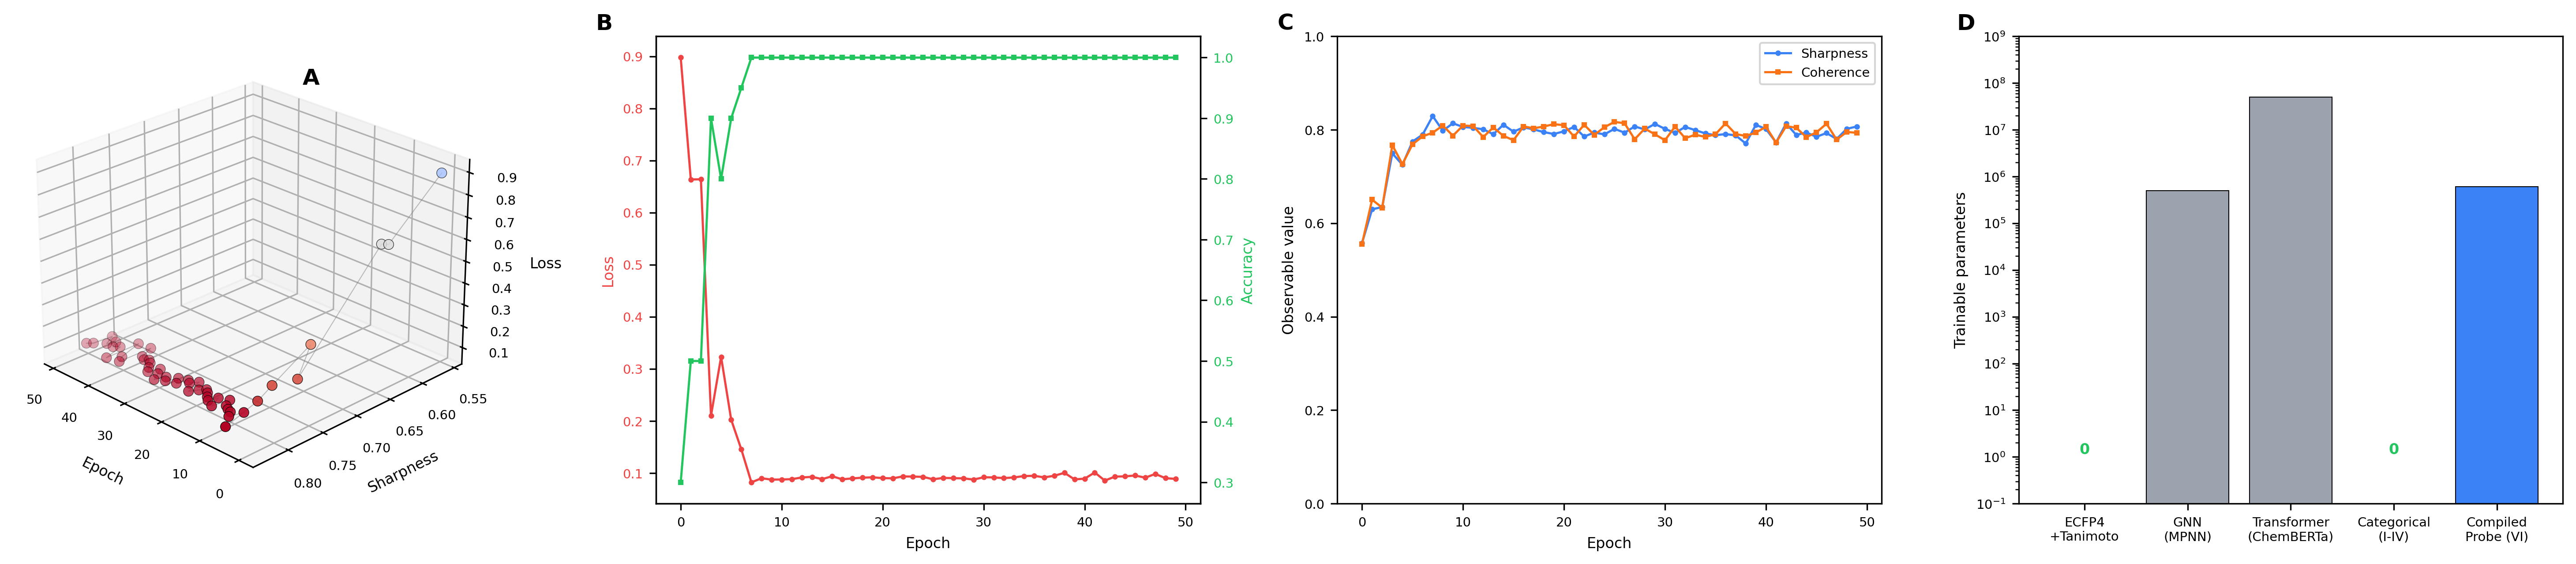
\includegraphics[width=\textwidth]{figures/panel_6_compiled_probe.png}
    \caption{\textbf{Model~VI: GPU-Supervised Compiled Probe.}
    (\textbf{A})~Three-dimensional training trajectory in (epoch, partition sharpness, loss) space. Points are coloured by accuracy (blue = low, red = high). The trajectory shows rapid descent from the high-loss, low-sharpness initialisation (epoch~0) to the low-loss, high-sharpness converged state (epoch~$\geq 3$). The single sharp transition reflects the probe learning to route queries to the correct categorical operation.
    (\textbf{B})~Training curves for loss (red, left axis) and routing accuracy (green, right axis) over 50 epochs. The loss drops by an order of magnitude within the first 3~epochs, after which accuracy saturates at 100\%. The compiled probe converges to perfect query routing using only 20 training queries and $\sim 0.6$M LoRA parameters---no human labels are required; the training signal comes entirely from GPU physical observables.
    (\textbf{C})~GPU physical observables---partition sharpness (blue) and phase coherence (orange)---over the training trajectory. Both observables rise sharply from $\sim 0.55$ (random initialisation) to $\sim 0.8$ (converged), tracking the accuracy improvement. The co-evolution of sharpness and coherence with accuracy confirms that optimising physical observation quality IS optimising answer quality (Triple Equivalence Theorem).
    (\textbf{D})~Trainable parameter count comparison across cheminformatics approaches on logarithmic scale. ECFP4+Tanimoto and categorical Models~I--IV have zero trainable parameters (marked with ``0''). Graph neural networks (GNNs, $\sim 10^5$--$10^6$) and transformers (ChemBERTa, $\sim 10^7$--$10^8$) require orders of magnitude more parameters. The compiled probe ($\sim 6 \times 10^5$) achieves natural-language routing at GNN-scale parameter cost, $\sim 100\times$ smaller than transformer approaches.}
    \label{fig:compiled_probe}
\end{figure*}
